\section{Практическое использование}

\subsection{Пример скрипта}
Типовой сценарий подготовки ролика: открыть файл, вырезать фрагмент,
убрать чёрные полосы, уменьшить разрешение и задать точную частоту кадров.
Соответствующий скрипт приведён в листинге 1.

\inputminted{text}{code/AviSynthScript.avs}

Комментарии начинаются с символа \verb|#| и игнорируются интерпретатором.
Для открытия контейнеров MP4 и MKV вместо \texttt{AviSource} применяется
функция \texttt{FFVideoSource} после загрузки плагина FFMS2 командой
\texttt{LoadPlugin}~\cite{ffms2}: встроенная \texttt{AviSource} понимает
лишь AVI с установленными VFW-кодеками~\cite{avisynth}.

\subsection{Базовые функции}
Функции, использованные в листинге 1, сведены в таблицу 1.

\begin{table}[H]
  \centering
  \small
  \begin{tabular}{|l|l|l|}
    \hline
    Функция & Назначение & Пример вызова \\
    \hline
    \texttt{FFVideoSource} & открыть видео любого контейнера & \texttt{FFVideoSource("clip.mkv")} \\
    \texttt{AviSource} & открыть AVI с VFW-кодеком & \texttt{AviSource("clip.avi")} \\
    \texttt{Trim} & оставить диапазон кадров & \texttt{Trim(120, 240)} \\
    \texttt{Crop} & обрезать края кадра & \texttt{Crop(0, 200, 0, -200)} \\
    \texttt{LanczosResize} & изменить разрешение & \texttt{LanczosResize(1280, 720)} \\
    \texttt{ConvertToYV12} & перевести в формат YV12 & \texttt{ConvertToYV12()} \\
    \texttt{AssumeFPS} & задать частоту кадров & \texttt{AssumeFPS(24000, 1001)} \\
    \hline
  \end{tabular}
  \caption{Базовые функции AviSynth}
\end{table}

\subsection{Связка с VirtualDub2}
Скрипт \texttt{.avs} открывается в VirtualDub2 как обычный видеофайл
(File "--- Open video file); окно программы с загруженным скриптом показано
на рисунке 1.

\begin{figure}[H]
  \centering
  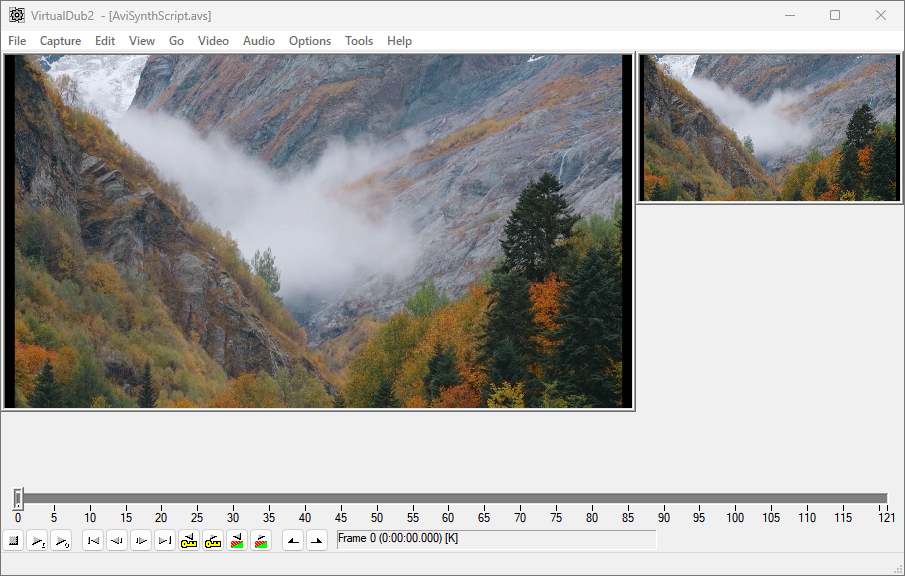
\includegraphics[width=0.9\textwidth]{images/openedscript.png}
  \caption{Скрипт AviSynthScript.avs, открытый в VirtualDub2}
\end{figure}

Дальнейшая обработка выполняется в одном из трёх режимов
(таблица 2).

\begin{table}[H]
  \centering
  \begin{tabular}{|l|l|}
    \hline
    Режим & Когда применяется \\
    \hline
    Direct stream copy & поток копируется без перекодирования \\
    Fast recompress & перекодирование без применения фильтров \\
    Full processing mode & полное применение фильтров и преобразований \\
    \hline
  \end{tabular}
  \caption{Режимы обработки видео в VirtualDub2~\cite{virtualdub}}
\end{table}

Результат работы фильтров кадрирования и масштабирования показан на
рисунке 2: слева "--- исходный кадр с чёрными полосами, справа "--- кадр
после применения \texttt{Crop} и \texttt{LanczosResize}.

\begin{figure}[H]
  \centering
  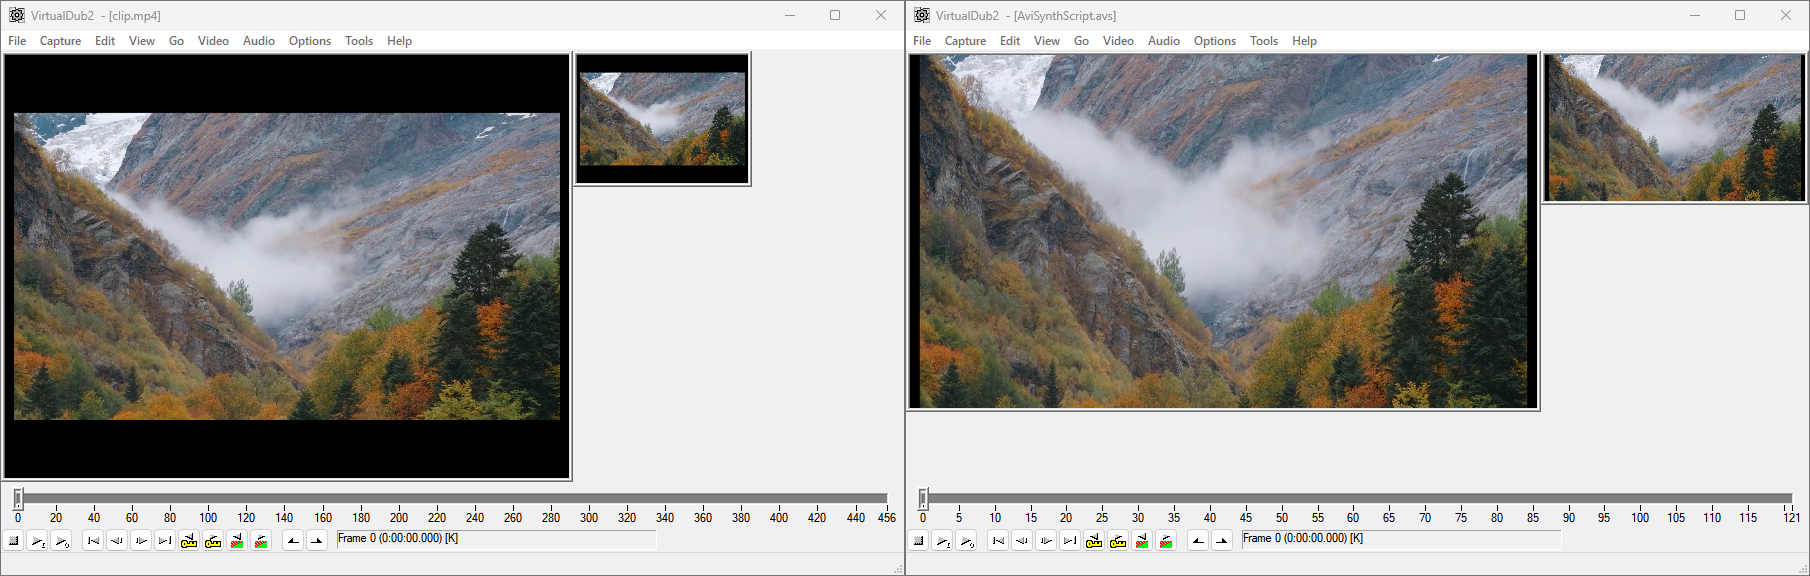
\includegraphics[width=0.96\textwidth]{images/beforeandafter.png}\hfill
  \caption{Кадр до и после применения фильтров кадрирования и масштабирования}
\end{figure}
